% \documentclass[a4paper,oneside]{article}
\documentclass[a4paper, 10pt, conference]{ieeeconf}
\IEEEoverridecommandlockouts
 % This command is only
  % needed if you want
  % to use the \thanks
  % command
\overrideIEEEmargins
% See the \addtolength command later in the file to balance the column lengths
% on the last page of the document

\usepackage[pdftex, pdftitle={DiagnosabilityVerification of Discrete-Event
Systems}, pdfauthor={Dmitry Myadzelets}, bookmarks=false,
% colorlinks=true, linkcolor=black
]{hyperref}

\usepackage{amsfonts, amssymb, amsmath} 
\usepackage{graphicx}
\usepackage{epstopdf}
\usepackage{tikz}
\usetikzlibrary{decorations.pathreplacing}
\usetikzlibrary{arrows,positioning,automata,shadows,fit,shapes}

\begin{document}

\title{How to Make a Discrete-Event System \\ Modularly Diagnosable}
\author{Dmitry Myadzelets$^{*,1,2}$, Andrea Paoli$^{1,3}$
\\ \today
\thanks{$^{1}$Center for Research on Complex Automated Systems (CASY), DEI,
University of Bologna, Viale Pepoli 3/2, 40123, Bologna, Italy}
	\thanks{$^{2}$E-mail: {dmitry.myadzelets@gmail.com}}
	\thanks{$^{3}$E-mail: {andrea.paoli@unibo.it}}
}
\maketitle

% To meet requirements of EU funding
% http://eacea.ec.europa.eu/about/eacea_logos_en.php "This project has been
% funded with support from the European Commission. This publication reflects
% the views only of the author, and the Commission cannot be held responsible
% for any use which may be made of the information contained therein."
\begin{figure}[!b]
\begin{tabular}{l p{60mm}}
 	
\includegraphics[height=10mm]{EU_flag.eps}
 	& \vspace{-10mm} \footnotesize
 	$^{*}$With the support of the Erasmus Mundus Action 2 programme of the
 	European Union.
\end{tabular}
\end{figure}

\begin{abstract}
This paper introduces an approach to achieve the modular diagnosability property
of a system by combining existing modules into new modules wich we call virtual
modules. A non-compositional analysis of the system is introduced, as a
preliminary step for the process of verification of the modular diagnosability
property. The analysis aimed to reduce the overall computational expenses. An
example of the approach is included.
\end{abstract}

\begin{keywords}
Discrete Event Systems, Modular Structure, Distributed Diagnosability
\end{keywords}

\newtheorem{assumption}{Assumption}
\newtheorem{definition}{Definition}
\newtheorem{conjecture}{Conjecture}
\newtheorem{lemma}{Lemma}
\newtheorem{corollary}{Corollary}
\newtheorem{example}{Example}
\newtheorem{theorem}{Theorem}

% %%%%%%%%%%%%%%%%%%%%%%%%%%%%%%%%%%%%%%%%%%%%%%%%%%%%%%%%%%%%%%%%%%%%%%%%%%%%%%
\section{Introduction}
% Raffly: What we are talking about and what problem exist there in general. How
% the problems are solved. What we suggest exactly and what is that for.
% How this paper is structured.

Discrete-Event Systems (DES) has successfully concurred significant area in the
systems engineering discipline due to their enormous capabilities of designing
and managing complex projects. While ``real-world'' systems are growing in scale
the solutions provided by DES have to evolve to tackle the increasing complexity
issues. For that reason the development of solutions relying on the fact that
the most of complex systems have naturally modular structure has been under
focus for the last two decades. Particularly, the task of design verification and
diagnosis with respect to undesired behaviour, commonly refereed as to faulty
behaviour of discrete systems, has a fairly developed theory nowadays.
In this paper we consider the automata framework for diagnosability analysis,
where a behaviour of DES is modeled by regular language and is represented
by automata.

Diagnosability analysis includes a verification if one can detect if the system
executes a faulty behaviour, i.e. a fault occurred, and a verification if one
can isolate a certain type of fault from other faults. This analysis implies
that the system's behaviour can be observed only partially. In DES built from more
then one modules it may be necessary to verify if the faults originated from one
module can be detected by observing only the same module, or by observing only
other modules, or under other implications with respect to the possible flow of
observations and their derivatives. Moreover, the verification of a modular
system is preferred to be done without composing its entire model from the
system's components since such composition may be not even feasible to perform
due to the correspondent computational expenses.

The approaches aimed to solve the problem of diagnosability verification
consider different architectures of DES and differ with respect to which of the
above implications they take into account. Either they require an entire model
of the system or not, what information is presented to each observation spot if
any, and etc. In this paper we use a classificaton as in
\cite{su_global_2005} where an approache is one of \emph{centralized},
\emph{decentralized} or \emph{distributed}.

The centralized approach was presented in \cite{sampath_diagnosability_1995}.
The authors consider a DES presented by one module, and they assume that all the
observations can be performed at one site. The diagnosability analysis of this
architecture is called the verification of centralized diagnosability. The paper
presents a procedure for such verification. Complexity of the procedure was
later improved in \cite{jiang_polynomial_2001} and
\cite{yoo_polynomial-time_2002}.

The decentralized approach, according to the above classification, exploits the
entire model built from its modules, and several local sites performing
observations. The sites may communicate in order to make a decision if a fault
has occurred. This architecture is presented in \cite{debouk_coordinated_1998},
\cite{qiu_decentralized_2006}, \cite{wang_diagnosis_2007} and others.

The distributed approach does not require to built the entire model of the
system. The architecture implies that the system has a set of observation spots,
and each spot observes only one module of the system. A communication among
observation spots is possible in order to make a decision about a fault
occurrence. The correspondent verification procedure checks if this architecture
is possible to apply for the given system. Such approach is presented in
\cite{su_distributed_2002}. The notion of modular diagnosability introduced in
\cite{contant_diagnosability_2006} meets the same architectural implications,
and we refer it as to the distributed diagnosability when the observation spots
do not communicate to each other.

In this paper we consider the distributed approach for a DES with modular
structure, i.e. no entire model of the system is presented and the fault
diagnosis procedure assumes that observation spots can not communicate. We
investigate the case when the system is not modular diagnosable initially, but
the modules of the system can be composed into \emph{virtual} modules in order
to force the modular diagnosability property. We study how to chose the system's
modules for the composition. For this goal a non-compositional analysis of the
system is introduced.
As the starting point we consider the definition of modular diagnosability
property and the correspondent verification algorithm from
\cite{contant_diagnosability_2006}. As far as we know no approach similar to our
has been published.

This paper is organized as follows. Section \ref{sec:Preliminaries} covers the
necessary notation and describes the diagnosability problem. Section
\ref{sec:Diagnosability} reviews diagnosability verification of a modular
system. In Section \ref{sec:Proposal} we focus on diagnosability by virtual
modules, and analysis of system's module structure with respect to the faulty
behaviour. The Section \ref{sec:Example} shows an example. The last Section
\ref{sec:Conclusion} concludes the current results and discuss possible
directions for further research.


%%%%%%%%%%%%%%%%%%%%%%%%%%%%%%%%%%%%%%%%%%%%%%%%%%%%%%%%%%%%%%%%%%%%%%%%%%%%%%%
% Move this picture to a place it looks better, if necessary.  
\begin{figure}[t]
\centering
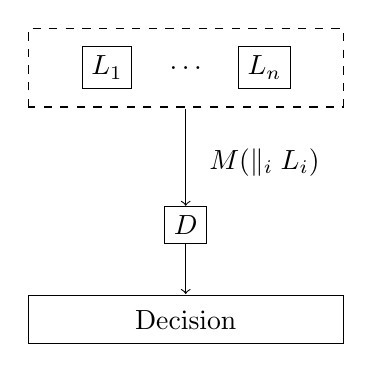
\begin{tikzpicture}
	\node[draw]		(0)	at (1, 3) 		{$L_1$};
	\node[]			(1)	[right of = 0]	{$\ldots$};
	\node[draw]		(2)	[right of = 1]	{$L_n$};
	\draw[dashed] (0, 2.5) rectangle (4, 3.5);
	\node[]			(3) at (2, 2.6) {};
	\node[draw]		(4) at (2, 1) {$D$};
	\draw[->] (3) -- (4);
	\node[]	at (3, 1.8) {$M(\parallel_{i} L_i)$};
	\node[]		(5) [below of = 4] {};
	\draw[->] (4) -- (5);
	\draw[] (0, -.5) rectangle (4, 0.1);
	\node[]			(3) at (2, -.2) {Decision};
\end{tikzpicture}
\caption{Architecture of a system with centralized diagnosis}
\label{fig_centralized}
\end{figure}

\begin{figure}[t]
\centering
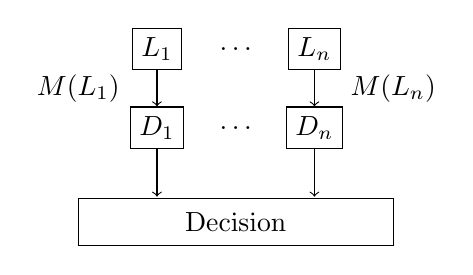
\begin{tikzpicture}
	\node[draw]		(0)	at (1, 2) 		{$L_1$};
	\node[draw]		(00) [below of = 0] {$D_1$};
	\node[]			(10) [below of = 00] {$$};
	\draw[->] (0) -- (00);
	\draw[->] (00) -- (10);

	\node[]			(1)	[right of = 0]	{$\ldots$};
	\node[]			(11)[right of = 00]	{$\ldots$};

	\node[draw]		(2)	[right of = 1]	{$L_n$};
	\node[draw]		(22) [below of = 2] {$D_n$};
	\node[]			(20) [below of = 22] {$$};
	\draw[->] (2) -- (22);
	\draw[->] (22) -- (20);

	\node[]	at (0, 1.5) {$M(L_1)$};
	\node[]	at (4, 1.5) {$M(L_n)$};

	\draw[] (0, -.5) rectangle (4, 0.1);
	\node[]			(3) at (2, -.2) {Decision};
\end{tikzpicture}
\caption{Architecture of a system with decentralized diagnosis}
\label{fig_decentralized}
\end{figure}

\begin{figure}[t]
\centering
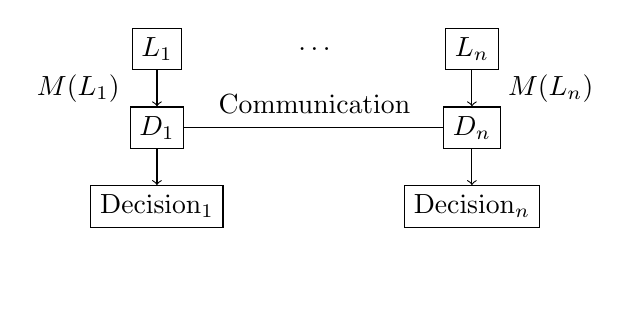
\begin{tikzpicture}
	\node[draw]		(0)	at (1, 2) 		{$L_1$};
	\node[draw]		(00) [below of = 0] {$D_1$};
	\node[draw]		(p0) [below of = 00] {Decision$_1$};
	\node[]			(10) [below of = p0] {$$};
	\draw[->] (0) -- (00);
	\draw[->] (00) -- (p0);

	\node[]			(1)	at (3, 2)	{$\ldots$};
	\node[] at (3, 1.3) {Communication};

	\node[draw]		(2)	at (5, 2) 		{$L_n$};
	\node[draw]		(22) [below of = 2] {$D_n$};
	\node[draw]		(p2) [below of = 22] {Decision$_n$};
	\node[]			(20) [below of = 22] {$$};
	\draw[->] (2) -- (22);
	\draw[->] (22) -- (p2);
	\draw[] (00) -- (22);

	\node[]	at (0, 1.5) {$M(L_1)$};
	\node[]	at (6, 1.5) {$M(L_n)$};
\end{tikzpicture}
\caption{Architecture of a system with distributed diagnosis}
\label{fig_distributed}
\end{figure}


%%%%%%%%%%%%%%%%%%%%%%%%%%%%%%%%%%%%%%%%%%%%%%%%%%%%%%%%%%%%%%%%%%%%%%%%%%%%%%%
\section{Preliminaries}
\label{sec:Preliminaries}
The notation used in this document is adopted from
\cite{cassandras_introduction_2010}.
Let $\Sigma$ be a finite set of events. A sequence of events is a string.
$\Sigma^*$ denotes a set of all finite strings over $\Sigma$.
$L\subseteq\Sigma^*$ is a language over $\Sigma$. Given strings $s$ and $t$,
$st$ is their concatenation. Given strings $s$ and $w$, $w$ is a prefix of $s$
if exists $t$ such that $wt = s$. Prefix closure of $L$, denoted by
$\overline{L}$ is a set of all prefixes of all strings in $L$.
If $\overline{L} = L$ then $L$ is prefix-closed. The post language of $L$ after
a string $s$ is denoted as $L/s$, i.e. $L/s = \{t\mid st \in L\}$. We
write $\sigma \in s$ if the event $\sigma \in \Sigma$ appears in the string $s
\in \Sigma^*$. If $\{s\}$ is a singleton, we write $s$ for operations on
languages.

An automaton $G$ is a tuple $$G=(X,\Sigma,\Delta,x_0, X_m),$$ where $X$ is a
set of states, $x_0 \in X$ is an initial state, $X_m \subseteq X$ is the set of
marked states, and $\Delta: X \times \Sigma \rightarrow X$ is the transition
function.
We say the a language $L = \mathcal{L}(G)$ is generated or recognized by the
automaton $G$. In this paper we assume that for each language there is always a
correspondent automaton, and vice versa. The marked language $L_m \subseteq L$
is intended to make a part of the automaton's behaviour distinguishable.

Some events of DES can not be observed. To reflect that the set of events
$\Sigma$ is partitioned into disjointed sets of observable events $\Sigma_o$ and
not observable events $\Sigma_{ou}$ such that $\Sigma = \Sigma_o~\dot{\cup}~
\Sigma_{ou}$.
The $M: \Sigma^* \rightarrow \Sigma_o^*$ denotes the natural projection that
erases unobservable events; $\epsilon$ means the empty string. The
correspondent inverse projection is $M^{-1}: \Sigma_o \rightarrow 2^\Sigma$. If
a set of events is partitioned into subsets, $\Sigma = \bigcup_i
\Sigma_{i} \mid i \in \mathbb{N}$, the natural projection over the partition
members is denoted as $M_i: \Sigma_i^* \rightarrow \Sigma_{i,o}^*$.

Let $I = \{1,2,\ldots,n\} \subset  \mathbb{N}$ be an index set. A system is
defined by a set of automata $\{G_{i \in I}\}$ and a correspondent set
of languages $\{L_{i \in I}\}$. We use the term \emph{local} in context
of the automata and languages from these sets. The \emph{global} language of the
system is thus defined by the parallel composition of its local languages: $L =
\parallel_{i \in I} L_i$.
The natural projection is commonly defined over Kleene closure on event sets.
We restrict it, for simplicity of notation, to the system's languages as
follows: $P_i(L) = \{s\mid s\in L_{i}\}$ and $P_i^{-1}(L_{i}) = \{s \mid s \in
L\}, ~i \in I$.


\subsection{Architectures for on-line diagnosis}
Architectures for on-line diagnosis of three tipes: centralized, decentralized
and distributed, can be stuctured as follows.

\subsubsection{Centralized}
The structure is depicted in Figure \ref{fig_centralized}. In this architecture
the global language is built by the parallel composition and then the diagnoser
$D$ introduced in \cite{sampath_diagnosability_1995} for the global language is
constructed. Upon the current state of the diagnoser a decision on the fault
occurrence is made.

\subsubsection{Decentralized}
In the approach only local diagnosers are built.
The diagnosers provide a necessary information (a protocol) to a central
decision node. The diagnosers do not communicate to each other. This
architecture is depicted in Figure \ref{fig_decentralized}.
Notable works on decentralized architecture are
\cite{debouk_coordinated_1998},
\cite{contant_diagnosability_2006} and \cite{wang_diagnosis_2007}.

\subsubsection{Distributed}
The architecture is depicted in Figure \ref{fig_distributed}.
Examples of a correspondent approach can be found in
\cite{pencole_formal_2005} and \cite{schumann_decentralised_2010}.


%%%%%%%%%%%%%%%%%%%%%%%%%%%%%%%%%%%%%%%%%%%%%%%%%%%%%%%%%%%%%%%%%%%%%%%%%%%%%%%
\section{Diagnosability of a Modular System}
\label{sec:Diagnosability}

%\subsection{Faulty and non-faulty languages}
Diagnosability analysis uses a notion of a faulty language to describe the
faulty behaviour of discrete-event system. This section discuses design issues
related to representations of the faulty language and focuses on a definition
of modular diagnosability.

The faulty behavior is usually modeled by introducing fault events or by faulty
specifications. We refer to this approaches as to \emph{event-based} and
\emph{specification-based} correspondingly. All the aforementioned works exploit
the event-based approach, whereas the works \cite{zhou_decentralized_2008} and
\cite{sartini_methodology_2010} are examples of the specification-based one.

In the event-based approach fault events are a special type of event, such that
$\Sigma_{uo}$ can be disjointed into the sets of faults $\Sigma_f$ and
non-faults $\Sigma_{uo}\backslash \Sigma_f$. A string containing a fault event
is called \emph{faulty string}. A set of faulty strings is called \emph{faulty
language}, i.e. formally 
$$L_f = \{ s \in L \mid \sigma \in s, \sigma \in \Sigma_f\}.$$ 
By definition, the faulty language is not necessarily prefix-closed in general,
$L_f \subseteq \overline{L_f}$. Thus, in the event-based approach the language
of the system can be partitioned into faulty and non-faulty languages, where the
\emph{non-faulty language} is defined as $L_{nf} = L \backslash L_f$.

In the case of the specification-based approach the faulty specification allows
us to define undesired behavior when the fault events are not necessarily
introduced. In this case this behaviour is represented by a marked language $L_f
= L_m \subseteq L$. 

Different types of undesired behaviours (or types of faults) are defined by
partitioning $\Sigma_f$ into subsets (not necessarily disjoint) or by several
faulty specifications for the same language. 

Generally, the faulty language defined in the event-based approach can be
considered as a faulty specification. Thus, we can assume that if fault events
are defined then faulty specifications can also be defined.
Consequently, a set of different types of faults requires a correspondent set of
specifications.
Thus, a method suitable for the specification-based approach implies that it can
be adopted for the event-based approach. In this paper, for the sake of
unification, we use specification-based approach. For this reason the
definitions of diagnosability originally developed by their authors for the
event-based approach are slightly modified with no loss of meaning.

For the sake of simplicity, in the following we assume that there is only one
type of fault, and that the language of the system is live.

We define \emph{diagnosability of the fault} as follows:
\begin{definition} 
\label{def:fault_is_diag}
The fault is diagnosable if there is no two strings
with the same observation such that one string is faulty and of arbitrary
cardinality, and second one is non-faulty, i.e. if the following holds true:
\end{definition}
\begin{equation}
\begin{array}{l}
	\forall(s \in L_f, t \in L_f/s) 
	\\
	(\exists n \in \mathbb{N})
	(|t| \geq n) 
	\\
	\left[ M(st) \cap M(L_{nf}) = \emptyset \right].
\end{array}
\end{equation}

We define \emph{diagnosability of the language} as follows:
\begin{definition}
The language is diagnosable if its all faults are diagnosable.
\end{definition}
The two above definitions altogether are similar to the Definition 1 in
\cite{sampath_diagnosability_1995}. We recall the statement in
\cite{contant_diagnosability_2006} proved by Theorem 2, that the global
language of the system is not diagnosable only if exists at least one non-diagnosable
local language. If all the local languages are diagnosable then the global
language is diagnosable. We refer to this property as to a local diagnosability
property:

\begin{definition}[Local diagnosability] Given the set of local languages
$\{L_{i \in I}\}$. The global language $L = \parallel L_i$ is
locally diagnosable if each local language $L_i$ is diagnosable, i.e. if
the following holds true:
\end{definition}
\begin{equation}
\begin{array}{l}
	\forall(i \in I, s \in L_{i,f}, t \in L_{i,f}/s)
	\\
	(\exists n \in \mathbb{N})
	(|t| \geq n)
	\\
	\left[ M_i(st) \cap M_i(L_{i,nf}) = \emptyset \right].
\end{array}
\end{equation}

A definition of modular diagnosability extends the definition of local
diagnosability as it takes into account the case when a faulty string locally
indistinguishable in one module becomes distinguishable due to the
composition with another module:

\begin{definition}[Modular diagnosability] Given the set of local languages
$\{L_{i \in I}\}$ and its correspondent sets $\{L_{i,f}\}$ and
$\{L_{i,nf}\}$. The global language $L = \parallel L_i$ is \emph{modularly
diagnosable} with respect to
$M_i: \Sigma^* \rightarrow \Sigma_{i,o}^*$ 
if the following holds true:
\end{definition}
\begin{equation}
\begin{array}{l}
	\forall(i \in I, s \in L_{i,f}, t \in L_{i,f}/s)
	\\
	(\exists n \in \mathbb{N})
	(|t| \geq n)
	\\
	\left[ M_i(P_i^{-1}(st)) \cap M_i(P_i^{-1}(L_{i,nf})) = \emptyset \right].
\end{array}
\end{equation}

It was proved in \cite{contant_diagnosability_2006} by Theorem 2, Part 2 
that the local diagnosability implies the modular diagnosability\footnote{In
\cite{zhou_decentralized_2008} the authors show that the local diagnosability
and modular diagnosability are not comparable but they have a different setup
for the problem.}, i.e.
\begin{equation}
\begin{array}{l}
	\forall(i \in I, s \in L_{i,f}, t \in L_{i,f}/s)
	\\
	(\exists n \in \mathbb{N})
	(|t| \geq n)
	\\
	\left[ M_i(st) \cap M_i(L_{i,nf}) = \emptyset \right]
	\Rightarrow 
	\\ 
	\left[ M_i(P_i^{-1}(st)) \cap M_i(P_i^{-1}(L_{i,nf})) = \emptyset \right].
\end{array}
\end{equation}


Recall the Definition \ref{def:fault_is_diag} of the diagnosable fault. If a
module is not diagnosable locally then exist at least two strings in its
language, one is faulty and one is not, with the same observation of arbitrary
length, i.e. the strings are \emph{not distinguashable}. This
indistinguishability can disappear if and only if:
$a)$ at least one string can be not in its language due to concurency with other
module, and then the strings would be distinguashable locally - the verification
of the modular diagnosability property is devoted to find if this is the case;
$b)$ indistinguishability is broken globally by interleaving sequences of the
module's events with observable events of other modules. The later case is
expressed in the following conjecture:
\begin{conjecture} Given two modules with languages $L_1$ and $L_2$, and the
global language of the system $L = L_1 \parallel L_2$. Suppose there is only one
faulty string $s \in L_1$ such that it is not distinguashable from at least one
string of $L_1\backslash s$. Thus, $L_1$ is not locally diagnosable. Suppose the
system is not modular diagnosable. Then the global language $L$ is diagnosable
only if all the strings $t \in P_1^{-1}(s)$ change their observation due to 
the composition with the language $L_2$.
\end{conjecture}

The above conjecture gives the insight into the underlining idea of our
approach. If we find a module which makes the faulty string distinguashable
then the composition of that module with a faulty one would result in a new
module satisfying the property of local diagnosability, thus improving
the modular diagnosability property of the system. In the following section we
provide a formal description of the problem.

% In the above the infinite length of the string $s$ is equal to the statement
% that the string $s$ forms a cycle. This definition is more weak then one
% presented in \cite{sampath_diagnosability_1995} because it does not assume non
% existence of unobservable cycles.


\section{Virtual Modules and Non-Compositional Analysis}
\label{sec:Proposal}

Our goal is to have the system modularly diagnosable. If the initial modularity
does not satisfy the property of modular diagnosability we assume that the set
of modules can be partitioned such that all the modules in each partition can be
considered as a \emph{virtual module}, and the system with the new modularity
satisfies the property of modular diagnosability.

\begin{definition}[Diagnosability of virtual modules] 
Let $I = \{1,2,\ldots,n\} \subset  \mathbb{N}$ be an index set, and $J$ be a
partition of $I$. Given the set of local languages $\{L_{i \in I}\}$ and its
corresponded subsets $\{L_{i,f}\}$ and $\{L_{i,nf}\}$. The global language $L =
\parallel L_i$ is modularly diagnosable with respect to
$M_j: \Sigma^* \rightarrow \Sigma_{j,o}^* 
\mid j \in J, ~\Sigma_{j,o} =\bigcup_{i \in j} \Sigma_{i,o}$ 
if the following holds true:
\end{definition}
\begin{equation}
\begin{array}{l}
	\forall(i \in I, s \in L_{i,f}, t \in L_{i,f}/s)
	\\
	(\exists n \in \mathbb{N})
	(|t| \geq n)
	\\
	\left[ M_j(P_i^{-1}(st)) \cap M_j(P_i^{-1}(L_{i,nf})) = \emptyset \right].
\end{array}
\end{equation}

If $\forall j \in J, L_{j} = \parallel L_{i \in j}$ then, by definition, $L =
\parallel L_{i \in I} = \parallel L_{j \in J}$, and all the statements related
to the modular diagnosability  property can be applied for the diagnosability by
virtual modules.

In order to find a partition of system's modules satisfying the modular
diagnosability property one may take a faulty module, enumerate all possible
sets of other modules, compose all the languages from each set with the faulty
language, and check the resulting language for modular diagnosability.
Such process is computationally expensive, since the number of possible
partitions $J$ is exponential with respect to the cardinality of $I$. However,
not each module can change diagnosability. We can significally decrease the
complexity by selecting only the modules which can probably change
diagnosability. For this purpose a procedure to check if an arbitrary module
potentially can change diagnosability, is required.

In the sequel, for the sake of simplicity, we suppose that the system consists
only of two modules with the correspondent languages $L_1$ and $L_2$. The
language of the system is $L = L_1 \parallel L_2$. Suppose that only one module
has a faulty behaviour: $L_1 = L_{1,f} ~\dot{\cup}~ L_{1,nf}$.
Suppose that $L_1$ is not diagnosable locally, but $L$ is diagnosable.

Firstly, we define the notion of observation changing of a string in a global
language.
\begin{definition}Given two languages $L_1$ and $L_2$. A string $s \in
L_1$ \emph{changes its observation} $M_1(s)$ in the language $L$ if
there is no the same observation in $P_1^{-1}(s)$, i.e.
if the following holds true:
\end{definition}
\begin{equation}
\label{def:obs}
\begin{array}{l}
	\left[ M(L) \cap M_1(s) = \emptyset \right].
\end{array}
\end{equation}

\begin{lemma}
\label{lem_changed_observation}
Given two languages $L_1$ and $L_2$, and a string $s \in L_1$.
Assume that $s \in P_1(L)$. The string $s$ changes its observation in the
language $L$ if and only if:
\end{lemma}
\begin{subequations}\label{lem:obs}
\begin{align}
	(\exists \sigma \in s \mid \sigma \in \Sigma_1 \cap \Sigma_2)
	\label{lem:obs1}
	\\
	(\forall t\sigma \in L_2)
	\left[M_2(t) \neq \emptyset \right],
	\label{lem:obs2}
	\\
	\textrm{where } M_2: \Sigma^* \rightarrow (\Sigma_{2,o} \backslash
	\Sigma_1)^*. 
	\label{lem:obs3}
\end{align}
\end{subequations}

\begin{proof}
In order to prove sufficiency of (\ref{lem:obs}) we use its converse relation
and prove by contradiction that the change of observation (\ref{def:obs}) is
necessary.
Assume $\exists w \in L$ and $\exists s \in L_1$ such that
$M(w)= M_1(s)$ and, hanceforce, (\ref{def:obs}) is false. Let $\exists
\sigma \in \Sigma_1 \cap \Sigma_2$ such that $\sigma \in w$ and also
(\ref{lem:obs1}) holds. Then may $\exists u \sigma \in \overline{w}$ such that
$M_2(u) = \emptyset$, and then $M_2(P_2(u)) =
\emptyset$ which contradicts (\ref{lem:obs2}). Now, let (\ref{lem:obs2})
be true for all $t\sigma \in P_2(w)$. Then the assumption $M(w)=
M_1(s)$ holds only if $\sigma \not \in s$, which contradicts (\ref{lem:obs1}). 

We prove necessity of (\ref{lem:obs}) by contradiction.
Let (\ref{lem:obs1}) holds, and $\exists t\sigma \in L_2$ such that
$M_2(t) = \emptyset$. Then may $\exists t'\sigma \in 
L \subseteq P_2^{-1}(t\sigma)$ such that $M_2(t') =
\emptyset$ and $M_1(t') = M_1(s) \neq \emptyset$, which contradicts
(\ref{def:obs}).
Now, let (\ref{lem:obs2}) holds and $\not \exists \sigma \in s' \in P_1^{-1}(s)
\mid \sigma \in \Sigma_1 \cap \Sigma_2$. Then may $\exists w \in L_2$ and,
hence, $w' \in L \subseteq P_2^{-1}(w)$ such that $M(w')=M(s)$,
which contradicts (\ref{def:obs}).
\end{proof}

Informally, the above lemma says that the string of the local language $L_1$
changes its observation in the global language $L$ if and only if the string has
an event in common with the language $L_2$, and all the strings of $L_2$ which
have this common event have observable events in the prefixes, and some of the
observable events in the prefixes are not common with $L_1$.

We call the subset of stings $\{t \in L_2\}$ satisfying condition
(\ref{lem:obs2}) as the \emph{adjacent observable support} for the given string
$s \in L_1$.

\begin{definition} Given two languages $L_1$ and $L_2$. We say that a string $s
\in L_{1}$ is distinguished from the all other local strings $L_1\backslash s$
in the language $L$ if the following holds true:
\end{definition}
\begin{equation}
\label{def:dist}
\begin{array}{l}
		M(s \parallel L_2) \cap M((L_1\backslash s) \parallel L_2)
		= \emptyset.
%   (\forall w \in L_1\backslash s)
%   	\left[ M(w \parallel L_2) \cap M(s\parallel L_2) = \emptyset \right].
\end{array}
\end{equation}

\begin{lemma}
\label{lem:distinguished}
Given two languages $L_1$ and $L_2$. Assume that $L_1 = P_1(L)$. The string $s
\in L_1$ is distinguished from $L_1\backslash s$ in the language $L$ if $s$ has
an adjacent observable support $L_{2,s} \subseteq L_2$ which
satisfies the following condition:
\end{lemma}
\begin{subequations}
\begin{align}
	(\forall t \in L_{2,s})
	(\exists \sigma \in t \mid \sigma \in \Sigma_1 \cap \Sigma_2)
	\label{lem:dist1}
	\\
	(\forall w \in L_1\backslash s)(\sigma \not \in w)
	\label{lem:dist2}
	\\
	(\forall t'\sigma \in \overline{t})
	[M_2(t / t'\sigma) \neq \emptyset]
	\label{lem:dist3},
\end{align}
\end{subequations}

where $M_2$ is defined as in (\ref{lem:obs3}). 

\begin{proof}
Assume (\ref{def:dist}) is false, i.e. $\exists w' \in P_1^{-1}(w)$ and $\exists
s' \in P_1^{-1}(s)$ such that $M(w') = M(s')$. 

Assume (\ref{lem:dist1}) and (\ref{lem:dist2}) hold. Then may $\exists t' \in
\overline{s'} \mid t' \in P_2^{-1}(L_{2,s})$ such that $M(t') = M(w')$, and $t =
P_2(t')$ such that $M_2(t) = M_2(w)$. And may $\exists t'' \in \overline{t}$
such that $M_2(t'') = M_2(w)$. Since $\sigma \in t$ and $\sigma \not \in w$,
then $M(t \backslash t''\sigma) = \emptyset$ for any $t''\sigma \in
\overline{t}$, which contradicts (\ref{lem:dist3}).

Assume (\ref{lem:dist1}) and (\ref{lem:dist3}) hold. Let $M_1(L_1) = \emptyset$
and $M_2(t\backslash t'\sigma) = M_2(s) = M_2(s)$. Then $\forall s' \in
M(P_1^{-1}(s))$ there exists $\sigma \in s'$, which contradicts
(\ref{lem:dist2}).

Assume (\ref{lem:dist2}) and (\ref{lem:dist3}) hold. If (\ref{def:dist}) is
false, then (\ref{lem:dist1}) is false. However, (\ref{lem:dist3}) is suffucient
for (\ref{lem:dist1}), which contradicts the former statement.
\end{proof}

Informally, the above lemma says that a string $s$ becomes distinguashable from
the other strings $L_1\backslash s$ in the global language, when the occurence
of events from the observable support happens only in $P^{-1}(s)$ due to
common events. Thus, whenever we observe events of the observable support of
$L_2$, we are sure the string $s$ in $L_1$ is being executed.


\begin{figure}[t]
\centering
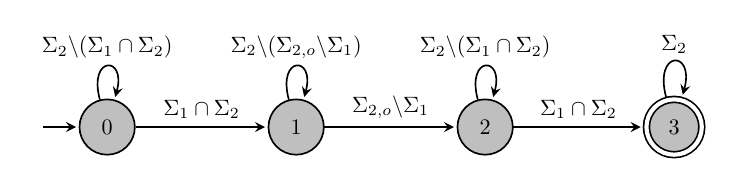
\begin{tikzpicture}
[->,>=stealth, node distance=30mm, auto, initial text=, shorten >=1pt,
semithick, 
every state/.style={fill=lightgray},
every node/.style={scale=0.8}, 
accepting/.style={double distance=1.5pt, outer sep=0.75pt+\pgflinewidth}
]
  \node[initial,state] (0)              {$0$};
  \node[state]         (1) [right of=0] {$1$};
  \node[state]         (2) [right of=1] {$2$};
  \node[state, accepting]         (3) [right of=2] {$3$};

  \path (0) edge [loop above] node {$\Sigma_2 \backslash (\Sigma_1 \cap \Sigma_2)$} (0)
  		(0) edge              node {$\Sigma_1 \cap \Sigma_2$} (1)
  		(1) edge [loop above] node {$\Sigma_2 \backslash (\Sigma_{2,o} \backslash \Sigma_1)$} (1)
        (1) edge              node {$\Sigma_{2,o} \backslash \Sigma_1$} (2)
  		(2) edge [loop above] node {$\Sigma_2 \backslash (\Sigma_1 \cap \Sigma_2)$} (2)
        (2) edge              node {$\Sigma_1 \cap \Sigma_2$} (3)
		(3) edge [loop above] node {$\Sigma_2$} (3)
%         (2) edge [bend left]  node {$\Sigma_1 \cap \Sigma_2$} (1)
        ;
\end{tikzpicture}
\caption{Automaton for marking the language $L_2$}
\label{fig:marking_L2}
\end{figure}

\begin{figure}[t]
\centering
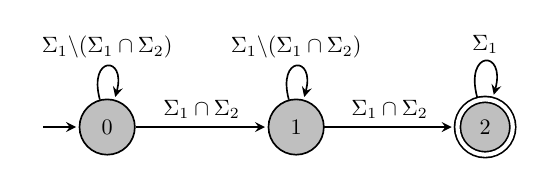
\begin{tikzpicture}
[->,>=stealth, node distance=30mm, auto, initial text=, shorten >=1pt,
semithick, 
every state/.style={fill=lightgray},
every node/.style={scale=0.8}, 
accepting/.style={double distance=1.5pt, outer sep=0.75pt+\pgflinewidth}
]
  \node[initial,state] (0)              {$0$};
  \node[state]         (1) [right of=0] {$1$};
  \node[state, accepting]         (2) [right of=1] {$2$};

  \path 
	(0) edge [loop above] node {$\Sigma_1 \backslash (\Sigma_1 \cap \Sigma_2)$} (0)
	(0) edge              node {$\Sigma_1 \cap \Sigma_2$} (1)
	(1) edge [loop above] node {$\Sigma_1 \backslash (\Sigma_1 \cap \Sigma_2)$} (1)
	(1) edge              node {$\Sigma_1 \cap \Sigma_2$} (2)
	(2) edge [loop above] node {$\Sigma_1$} (2)
% 	(1) edge [bend left]  node {$\Sigma_1 \cap \Sigma_2$} (0)
    ;
\end{tikzpicture}
\caption{Automaton for marking the language $L_1$}
\label{fig:marking_L1}
\end{figure}

As it was discussed in the Section \ref{sec:Diagnosability}, indistingushability
can be changed either by blocking the string in the local language due to
concurrency or by interleaving with observable events in other languages. Under
assumption that the all strings are not affected by concurrency, i.e. $L_1 =
P_1(L)$ we can state that the conditions of Lemma \ref{lem:distinguished} are
also necessary for changing distinguishability. For the sake of brevity no proof is
provided here.

The Figure \ref{fig:marking_L2} depicts an automaton which
accepts the sublanguage of $L_2$ satisfying conditions (\ref{lem:obs1}),
(\ref{lem:dist1}) and (\ref{lem:dist3}) of the above lemmas.
The Figure \ref{fig:marking_L1} depicts an automaton which
marks a sublanguage of $L_1$ satisfying conditions (\ref{lem:obs1}) and
(\ref{lem:dist1}). 

A procedure verifying if a string $s \in L_1$ is distinguashable in the global
language $L$ consists of two steps. First, the string $s$ should be marked by
the automaton depicted in the Figure \ref{fig:marking_L1}. The set of common
events $\Sigma_1 \cap \Sigma_2$ is reduced to the set of events causing
transitions in the automaton. Second, all the continuations of the strings of
the language $L_2$ which have these common events should be accepted by the
automaton depicted in the Figure
\ref{fig:marking_L2}.

Now we are ready to apply Lemma \ref{lem:distinguished} with respect to
diagnosability property, but make some notes before. Intuitively, one
would apply the conditions of the lemma for faulty and non-faulty
languages. Recall also, that faulty and non-faulty languages are disjoint.
However, since the faulty language is not prefix-closed in general, its prefix
can be a part of the prefix of the non-faulty language, i.e. $\overline{L_{i,f}}
\cap L_{i,nf} \neq \emptyset$. Changing observability of the
sublanguage $\overline{L_{i,f}} \cap L_{i,nf}$ has no effect for diagnosability.
Nence, we exclude this sublanguage from the conditions verification
procedure.

\begin{lemma}
\label{lem:diagnosable}
Given $L_1, L_2$, $L_{1,f} \subseteq L_1$ and $L_{1,nf} \subseteq L_1$. A
language $L = L_1 \parallel L_2$ is diagnosable if $L_{1,f}$ or $L_{1,nf}
\backslash \overline{L_{1,f}}$ has an observable support in $L_2$, which
satisfies conditions \ref{lem:dist1}-\ref{lem:dist3}.
\end{lemma}

Clearly, the automata depicted in Figures \ref{fig:marking_L2} and
\ref{fig:marking_L1} can not be simply used in a procedure verifying
diagnosability, since we should avoid the verification of $\overline{L_{1,f}}
\backslash L_{1,f}$ and $L_{1,nf} \backslash \overline{L_{1,f}}$. We leave
development of such procedure for furture work. However, the automata can be
used to demonstrate the approach in a trivial case, as it is shown in the next
section.

%%%%%%%%%%%%%%%%%%%%%%%%%%%%%%%%%%%%%%%%%%%%%%%%%%%%%%%%%%%%%%%%%%%%%%%%%%%%%%%
\section{Example}
\label{sec:Example}

Consider the system of two automata $G_1$ and $G_2$ depicted in Figure
\ref{fig:G1} and Figure \ref{fig:G2}. The set of events for the system is
$\Sigma = \{a, b, c, e, f\}$. Suppose the observable events are $\Sigma_o = \{c,
e\}$, and the set of faut events is $\{f\}$. Thus, only the language $L_1$ has a
fault, and $L_2$ has not. We use the verifier \cite{yoo_polynomial-time_2002} to
check if a language is diagnosable. The verifier for the language $L_1$ is
depicted in the Figure \ref{fig:verifier_G1}. One can check that it has an
indeterminate cycle.
The strings $fbc^*$ and $ac^*$ are not distinguashable in the local language
$L_1$. Hence, $L_1$ is not locally diagnosable.

We now use the verification procedure described in this paper to check if the
language $L_2$ can changes observation of either strings $fbc^*$ or
$ac^*$ in the language $L_1 \parallel L_2$ such that the strings become
distinguashable. The set of events common for $L_1$ and $L_2$ is $\{b, c\}$. It
can be verified that only the strings $fbc^*$ are marked by the automaton
depicted in the Figure \ref{fig:marking_L1}. Next, it can be verified that all
the strings of $L_2$ which have events common with the strings $fbc^*$ are
accepted by the automaton depicted in the Figure \ref{fig:marking_L2}. Thus, we
conclude that $L_2$ changes observation of the strings $fbc^*$ in the virtual
module $G$ built of modules $G_1$ and $G_2$, such that $G$ becomes diagnosable.
Indeed, if we make a parallel composition of the modules and build a verifier
for the result as it is depicted in the Figure \ref{fig:verifier_G1G2}, it can
be checked that the verifier has no indeterminate cycles.

\begin{figure}[t]
\centering
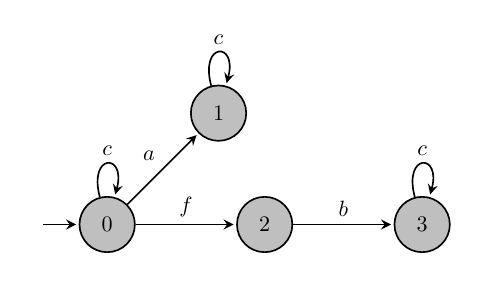
\begin{tikzpicture}
[->,>=stealth, node distance=25mm, auto, initial text=, shorten >=1pt,
semithick, 
every state/.style={fill=lightgray},
every node/.style={scale=0.8}, 
accepting/.style={double distance=1.5pt, outer sep=0.75pt+\pgflinewidth}
]
  \node[initial,state]		(0)              		{$0$};
  \node[state ]   (1) [above right of=0]	{$1$};
  \node[state]         		(2) [right of=0]		{$2$};
  \node[state]	(3) [right of=2]		{$3$};

  \path
 	(0) edge [loop above] node {$c$} (0)
 	(0) edge              node {$a$} (1)
 	(1) edge [loop above] node {$c$} (1)
 	(0) edge              node {$f$} (2)
 	(2) edge              node {$b$} (3)
 	(3) edge [loop above] node {$c$} (3)
    ;
\end{tikzpicture}
\caption{Automaton $G_1$}
\label{fig:G1}
\end{figure}

\begin{figure}[t]
\centering
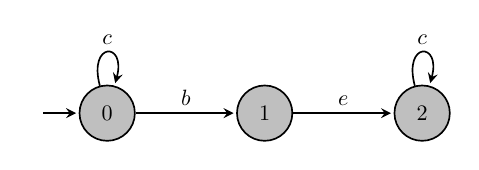
\begin{tikzpicture}
[->,>=stealth, node distance=25mm, auto, initial text=, shorten >=1pt,
semithick, 
every state/.style={fill=lightgray},
every node/.style={scale=0.8}, 
accepting/.style={double distance=1.5pt, outer sep=0.75pt+\pgflinewidth}
]
  \node[initial,state]		(0)              		{$0$};
  \node[state]         		(1) [right of=0]		{$1$};
  \node[state]	(2) [right of=1]		{$2$};

  \path
%  	(0) edge              node {$a$} (1)
 	(0) edge [loop above] node {$c$} (0)
 	(0) edge              node {$b$} (1)
 	(1) edge              node {$e$} (2)
 	(2) edge [loop above] node {$c$} (2)
    ;
\end{tikzpicture}
\caption{Automaton $G_2$}
\label{fig:G2}
\end{figure}

% It is a nice looking version of the verifier below, but its caption
% disappears when the Figure is shown. Strange...
 
% \begin{figure}[t]
% \centering
%  	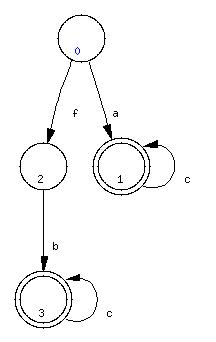
\includegraphics[height=50mm]{G1.jpg}
%  	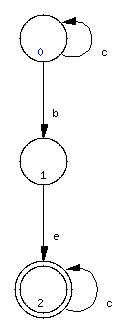
\includegraphics[height=50mm]{G2.jpg}
% \caption{Automata $G_1$ and $G_2$}
% \label{fig:G1_and_G2}
% \end{figure}
% 
% \begin{figure}[t]
% \centering
% \begin{tikzpicture}
% [->,>=stealth, node distance=20mm, auto, initial text=, shorten >=1pt,
% semithick, 
% every state/.style={fill=lightgray},
% every node/.style={scale=0.8}, 
% accepting/.style={double distance=1.5pt, outer sep=0.75pt+\pgflinewidth}
% ]
%   \node[initial,state]		(0N0N)             			{0N,0N};
%   \coordinate[below of=0N0N](fake);
%   \node[state]         		(2F0N) [left of=fake]		{2F,0N};
%   \node[state]         		(1N0N) [right of=fake]		{1N,0N};
%   \node[state]         		(3F0N) [below of=2F0N]		{3F,0N};
%   \node[state]         		(2F2F) [left of=3F0N]		{2F,2F};
%   \node[state]         		(1N2F) [right of=3F0N]		{1N,2F};
%   \node[state]         		(1N1N) [right of=1N2F]		{1N,1N};
%   \node[state]         		(3F2F) [below of=3F0N]		{3F,2F};
%   \node[state]         		(1N3F) [below of=1N2F]		{1N,3F};
%   \node[state]         		(3F3F) [below of=3F2F]		{3F,3F};
% 
%   \path
%   	(0N0N) edge              node {$f$} (2F0N)
%   	(0N0N) edge              node {$a$} (1N0N)
%   	(2F0N) edge              node {$f$} (2F2F)
%   	(2F0N) edge              node {$b$} (3F0N)
%   	(2F0N) edge              node {$a$} (1N2F)
%   	(1N0N) edge              node {$f$} (1N2F)
%   	(1N0N) edge              node {$a$} (1N1N)
%  	(1N1N) edge [loop right] node {$c$} (1N1N)
%   	(2F2F) edge              node {$b$} (3F2F)
%   	(3F0N) edge              node {$f$} (3F2F)
%   	(3F0N) edge              node {$a$} (1N3F)
%   	(1N2F) edge              node {$b$} (1N3F)
%   	(1N3F) edge [loop right] node {$c$} (1N3F)
%   	(3F2F) edge              node {$b$} (3F3F)
%   	(3F3F) edge [loop right] node {$c$} (3F3F)
%     ;
% \end{tikzpicture}
% \caption{Verifier of $G_1}
% \label{fig:verifier_G1}
% \end{figure}

\begin{figure}[t]
\centering
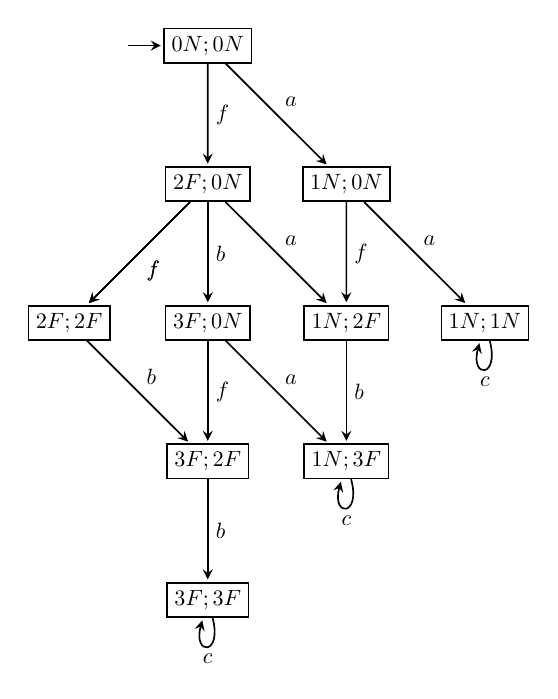
\begin{tikzpicture}
[->,>=stealth, node distance=22mm, auto, initial text=, shorten >=1pt,
semithick, 
every node/.style={scale=0.8}, 
accepting/.style={double distance=1.5pt, outer sep=0.75pt+\pgflinewidth}
]
  \node[draw, initial](0N0N)              	  {$0N;0N$};
  \node[draw]         (2F0N) [below of =0N0N] {$2F;0N$};
  \node[draw]         (1N0N) [right of =2F0N] {$1N;0N$};
  \node[draw]         (3F0N) [below of =2F0N] {$3F;0N$};
  \node[draw]         (2F2F) [left of =3F0N]  {$2F;2F$};
  \node[draw]         (1N2F) [right of =3F0N] {$1N;2F$};
  \node[draw]         (1N1N) [right of =1N2F] {$1N;1N$};
  \node[draw]         (1N3F) [below of =1N2F] {$1N;3F$};
  \node[draw]         (3F2F) [below of =3F0N] {$3F;2F$};
  \node[draw]         (3F3F) [below of =3F2F] {$3F;3F$};

  \path 
	(0N0N) edge	node {$f$} (2F0N)
	(0N0N) edge	node {$a$} (1N0N)
	(2F0N) edge	node {$f$} (2F2F)
	(2F0N) edge	node {$f$} (2F2F)
	(2F0N) edge	node {$b$} (3F0N)
	(2F0N) edge	node {$a$} (1N2F)
	(1N0N) edge	node {$f$} (1N2F)
	(1N0N) edge	node {$a$} (1N1N)
	(1N1N) edge [loop below] node {$c$} (1N1N)
	(2F2F) edge	node {$b$} (3F2F)
	(3F0N) edge	node {$f$} (3F2F)
	(3F0N) edge	node {$a$} (1N3F)
	(1N2F) edge	node {$b$} (1N3F)
	(3F2F) edge	node {$b$} (3F3F)
	(3F3F) edge [loop below] node {$c$} (3F3F)
	(1N3F) edge [loop below] node {$c$} (1N3F)
    ;
\end{tikzpicture}
\caption{Verifier of $G_1$}
\label{fig:verifier_G1}
\end{figure}

% \begin{figure}[t]
% \centering
%  	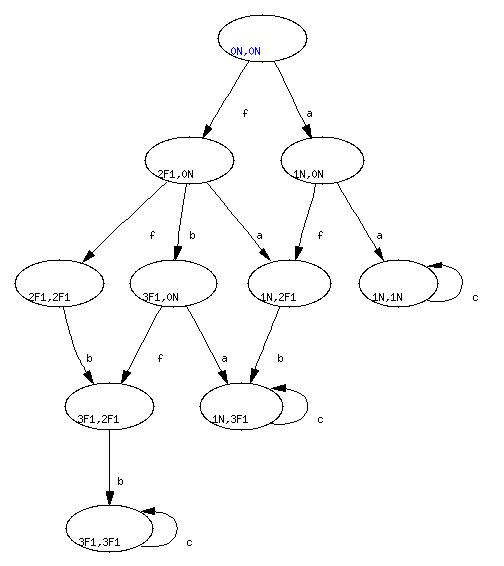
\includegraphics[height=80mm]{verifier_G1.jpg}
% \caption{Verifier of $G_1$}
% \label{fig:verifier_G1}
% \end{figure}

\begin{figure}[t]
\centering
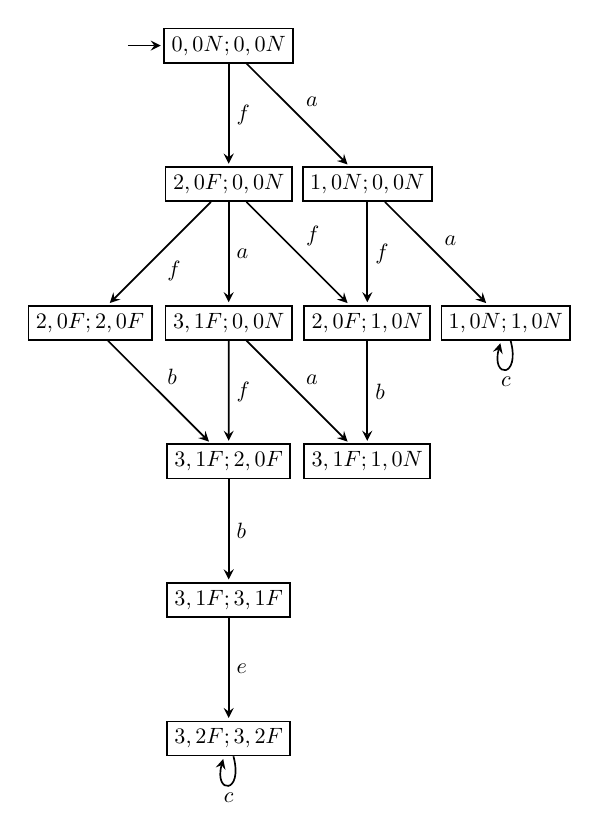
\begin{tikzpicture}
[->,>=stealth, node distance=22mm, auto, initial text=, shorten >=1pt,
semithick, 
every node/.style={scale=0.8}, 
accepting/.style={double distance=1.5pt, outer sep=0.75pt+\pgflinewidth}
]
  \node[draw, initial](00N00N)              	  {$0,0N;0,0N$};
  \node[draw]         (20F00N) [below of =00N00N] {$2,0F;0,0N$};
  \node[draw]         (10N00N) [right of =20F00N] {$1,0N;0,0N$};
  \node[draw]         (31F00N) [below of =20F00N] {$3,1F;0,0N$};
  \node[draw]         (20F20F) [left of =31F00N]  {$2,0F;2,0F$};
  \node[draw]         (20F10N) [right of =31F00N] {$2,0F;1,0N$};
  \node[draw]         (10N10N) [right of =20F10N] {$1,0N;1,0N$};
  \node[draw]         (31F20F) [below of =31F00N] {$3,1F;2,0F$};
  \node[draw]         (31F10N) [below of =20F10N] {$3,1F;1,0N$};
  \node[draw]         (31F31F) [below of =31F20F] {$3,1F;3,1F$};
  \node[draw]         (32F32F) [below of =31F31F] {$3,2F;3,2F$};

  \path
	(00N00N) edge	node {$f$} (20F00N)
	(00N00N) edge	node {$a$} (10N00N)
	(20F00N) edge	node {$f$} (20F20F)
	(20F00N) edge	node {$f$} (20F10N)
	(20F00N) edge	node {$a$} (31F00N)
	(10N00N) edge	node {$f$} (20F10N)
	(10N00N) edge	node {$a$} (10N10N)
	(10N10N) edge [loop below] node {$c$} (10N10N)
	(20F20F) edge	node {$b$} (31F20F)
	(31F00N) edge	node {$f$} (31F20F)
	(31F00N) edge	node {$a$} (31F10N)
	(20F10N) edge	node {$b$} (31F10N)
	(31F20F) edge	node {$b$} (31F31F)
	(31F31F) edge	node {$e$} (32F32F)
	(32F32F) edge [loop below] node {$c$} (32F32F)
    ;
\end{tikzpicture}
\caption{Verifier of $G_1 \parallel G_2$}
\label{fig:verifier_G1G2}
\end{figure}

% \begin{figure}[t]
% \centering
% 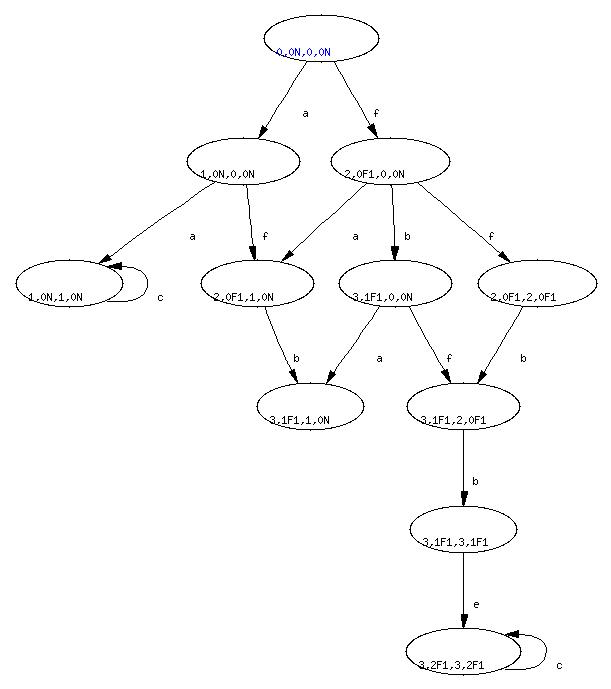
\includegraphics[height=100mm]{verifier_G1G2.jpg}
% \caption{Verifier of $G_1 \parallel G_2$}
% \label{fig:verifier_G1G2}
% \end{figure}


\addtolength{\textheight}{-0.5cm}
%%%%%%%%%%%%%%%%%%%%%%%%%%%%%%%%%%%%%%%%%%%%%%%%%%%%%%%%%%%%%%%%%%%%%%%%%%%%%%%
\section{Conclusion}
\label{sec:Conclusion}

In this paper we introduced a notion of virtual modules for DES, and proposed a
new definition of modular diagnosability by virtual modules. The approach
suggestes to combine the existing modules of the system into virtual modules in
a way that the system with the new modularity is modular diagnosable.

We introduced a non-compositional analysis of the system's modules, which allows
to verifiy if one module may change its observation by composition with others,
and if another module can change the obsevation of other modules. We defined
correspondent suffucient and necessary conditions for the modules' languages. If
the languages satisfy those conditions then one can state that the system can
be made modular diagnosable by creating virtual modules.
The suggested verificaion procedure has linear complexity with respect to the
number of states of a module.

We leave for the future work the problem of defining criteria of how to select
the best candidates for creating the virtual modules, what the optimal
partition of the set of the modules can be, and generalization of the problem.

% This command serves to balance the column lengths on the last page of the
% document manually. It shortens the textheight of the last page by a suitable
% amount. This command does not take effect until the next page so it should come
% on the page before the last. Make sure that you do not shorten the textheight
% too much.

\bibliographystyle{IEEEtran}
\bibliography{References}


% Feel free to remove the following text.
% \newpage

% 
% \subsection{}
% \begin{enumerate}
%   \item Do not consider non-compositional analysis first;
%   \item Global consistency = local observations after the parallel
%   composition, $\{ P_{I,i}(\parallel_{j \in I}M_i)\}$;    
%   
% \end{enumerate} 
% 
% Our heuristic is that we can tune the order the components are composed to lower
% the computational expenses. During an iterative process of the composition the
% following questions should be answered:
% \begin{enumerate}
%   \item Is there a way to analyse the system with respect to diagnosability with
%   no composition involved (non-compositional analysis)?
%   \item Given a non-diagnosable module and an adjacent one, should we take
%   the last one as a candidate for the composition?
%   \item If we have two modules can be taken which might be preferred to be
%   composed first?
% \end{enumerate}
% 
% Answers are given in the sequel.
% 
% % \section{Non-compositional analysis}
% % Non-compositional analysis should be the fist necessary step
% % to decide whether the system is not-diagnosable, before we start potentially more
% % computationally expensive compositional analysis. This step can be found in
% % some works but it is not considered as a separate topic there. A couple of works
% % is reviewed further.
% % 
% % In the work \cite{debouk_modular_2002} the authors study modular approach
% % aimed to decide in an incremental fashion if a global system is diagnosable. In
% % the Theorem 3.1 they state that the system is diagnosable if each module is
% % diagnosable. In the authors' verification algorithm the first step may be
% % referred as to the non-compositional analysis. The step can be describe as
% % follows: for each module check if it has indeterminate cycle in its diagnoser.
% % If there is no such cycle then the system is diagnosable. 
% % 
% % The non-compositional analysis equal to the above is presented in the work
% % \cite{contant_diagnosability_2006}. The authors study modular diagnosability,
% % and criteria for the system to be non-diagnosable is the existence of
% % an indeterminate cycle. They establish the following results: 
% % ``(a) if an indeterminate cycle exists in the monolithic diagnoser then
% % necessarily one of the local diagnosers contains an indeterminate cycle; 
% % (b) if none of the local diagnosers contains an indeterminate cycle then the
% % monolithic diagnoser does not contain an indeterminate cycle; and 
% % (c) if an indeterminate cycle exists in a local diagnoser then it may or may not
% % exist in the monolithic diagnoser''.
% % The cases (a) and (b) can be referred as to the non-compositional analysis, and
% % the correspondent step of checking each module for an indeterminate
% % cycle in its diagnoser is provided by the authors in the Algorithm 1.
% % 
% % It can be seen from the above, that the non-compositional analysis has
% % been limited only for checking of indeterminate cycle. In the following we
% % extend the non-compositional analysis and provide additional conditions for
% % diagnosability. Firstly we consider analysis of a module the faulty
% % behavior originates from, then we consider analysis of its adjacent modules.  
% 
% 
% %%%%%%%%%%%%%%%%%%%%%%%%%%%%%%%%%%%%%%%%%%%%%%%%%%%%%%%%%%%%%%%%%%%%%%%%%%%%%%%
% \subsection{Analysis of a module with a faulty behaviour}
% In this section we define sufficient and necessary conditions for diagnosability
% by analysing only the module with a faulty behaviour.
% 
% Given a system $G$ with two modules $\{G_1, G_2\}$ and
% their languages $\{L_1, L_2\}$. The language of the system is $L = L_1 \parallel
% L_2$. 
% The language of each module is partitioned into faulty $L_{i,f}\mid i\in
% \{1,2\}$ and non-faulty $L_i\backslash L_{i,f}$ languages.
% 
% % In cases when definition of diagnosability does not require any bounds for
% % faults to be detected, the sufficient condition for diagnosability is the
% % condition when no indeterminate cycle exists in any module. 
% % It is expressed in the following theorem (adopted from the aforementioned works)
% % under assumption that the languages are live:
% % \begin{theorem}[Sufficient condition for diagnosability]
% % \label{trm_sufficient_for_diag}
% % \begin{equation}
% % \begin{array}{l}
% % 	L \textrm{ is }D \Rightarrow 
% % 	\\[1ex]
% % 	\forall i \in |\{L_i\}|
% % 	\\[1ex]
% % 	\textrm{there is no indeterminate cycle in } Diag(L_i)
% % \end{array}
% % \end{equation}
% % \end{theorem}
% 
% % \begin{conjecture}[Sufficient condition for non-diagnosability]
% % If $\overline{L_{i,f}}$ has neither observable nor common events, then the
% %   system is not diagnosable, i.e:
% % \begin{equation}
% % \begin{array}{l}
% % 	(\forall s \in \overline{L_{i,f}}) 
% % 	(P_{i,j}(s) = \epsilon \land \textrm{ and }
% % 	M(s) = \epsilon) \Rightarrow L \textrm{ not }D,
% % 	\\[1ex] 
% % 	or, equally:
% % 	\\[1ex]
% % 	P_{i,j}(\overline{L_{i,f}}) = \emptyset \textrm{ and }
% % 	M(\overline{L_{i,f}}) = \emptyset \Rightarrow L \textrm{ not }D.
% % \end{array}
% % \end{equation}
% % \end{conjecture}
% % 
% % \begin{corollary}[Necessary condition for diagnosability] The system is
% % diagnosable only if at least one string in $\overline{L_{i,f}}$ has common or
% % observable events, i.e:
% % \begin{equation}
% % \begin{array}{l}
% % 	L \textrm{ is }D \Rightarrow \exists s \in \overline{L_{i,f}} \mid 
% % 	P_{i,j}(s) \neq \epsilon \textrm{ or } M(s) \neq \epsilon,
% % 	\\[1ex]
% %  	or, equally:
% % 	\\[1ex]
% % 	L \textrm{ is }D \Rightarrow
% % 	P_{i,j}(\overline{L_{i,f}}) \neq \emptyset \textrm{ or }
% % 	M(\overline{L_{i,f}}) \neq \emptyset 
% % \end{array}
% % \end{equation}
% % \end{corollary}
% 
% % (this condition implies the former conjecture, so no need for the above one)
% 
% We augment the above sufficient condition for diagnosability by a sufficient
% condition for non-diagnosability and the following necessary condition for
% diagnosability.
%  \begin{conjecture}[Sufficient condition for non-diagnosability]
% If $\exists s \in L_f$ which has no observable events, and $\overline{s}$ has no
% common events, then the system is not diagnosable, i.e:
% \begin{equation}
% \begin{array}{l}
% 	(\exists s \in L_{i,f}) 
% 	\left[
% 		P_{i,j}(\overline{s}) = \epsilon
% 	\right]
% 		\land
% 	\left[
% 		M(s) = \epsilon
% 	\right]
% 	\\[1ex]
% 	\Leftrightarrow
% 	\\[1ex]
% 	\left[
% 		P^{-1}_{i,j}P_{i,j}(\overline{L_{i,f}})\cap \overline{L_{i,f}} = \emptyset
% 	\right]
% 		\land
% 	\left[
% 		M^{-1}M(L_{i,f})\cap L_{i,f} = \emptyset
% 	\right]
% 	\\[2ex]
% 	\Rightarrow L \textrm{ not }D.
% \end{array}
% \end{equation}
% \end{conjecture}
% 
% \begin{corollary}[Necessary condition for diagnosability] The system is
% diagnosable only if all strings in $L_{i,f}$ have observable, and/or
% $\overline{s}$ have common events, i.e:
% \label{col_necessary}
% \begin{equation}
% \begin{array}{l}
% 	L \textrm{ is }D \Rightarrow 
% 	\\[2ex]
% 	(\forall s \in L_{i,f}) 
% 	\left[
% 		P_{i,j}(\overline{s}) \neq \epsilon
% 	\right]
% 		\lor 
% 	\left[
% 		M(s) \neq \epsilon 
% 	\right]
% 	\\[1ex]
% 	\Leftrightarrow
% 	\\[1ex]
% 	\left[
% 	P^{-1}_{i,j}P_{i,j}(\overline{L_{i,f}})\cap \overline{L_{i,f}} = \emptyset 
% 	\right]
% 		\lor
% 	\left[
% 		M^{-1}M(L_{i,f})\cap L_{i,f} = \emptyset
% 	\right]. 
% \end{array}
% \end{equation}
% \end{corollary}
% 
% \begin{example} This example shows how the non-compositional analysis might be
% organised.
% Lets consider the languages depicted in Figure \ref{fig_automaton_F-NF}.
% Assume the language presents one module of the system, and that other modules
% are diagnosable. It is clear that the language $L$ has only two cycles, formed
% by events $b$ and $c$ in states 4 and 5 respectively.
% Both cycles are presented in the faulty and non-faulty languages after
% partitioning. Hence the cycles are the candidates for indeterminate cycles in a
% diagnoser (for simplicity we omit construction of diagnosers here). 
% 
% According to the Theorem \ref{trm_sufficient_for_diag}, for the system to be 
% diagnosable it is sufficient do not have an indeterminate cycle in a diagnoser
% of this module. It is intuitive that the only chance to break
% possible indistinguishable strings is to block execution of faulty strings
% or to make them observable.
% 
% If the event $e$ is not observable, then according to the Corollary
% \ref{col_necessary}, some events in the prefix-closure of the faulty strings
% have to be common with at least one other module of the system to be blocked, or
% to make these strings distinguishable. Otherwise we can state that the system
% is not diagnosable.
% \end{example}
% 
% % \begin{conjecture}[Sufficient condition for diagnosability]
% % \begin{equation}
% % \begin{array}{l}
% % 	\forall i \in |\{L_i\}|
% % 	\\
% % 	P_{i,j}(L_{i,f}) = \emptyset \textrm{ and } 
% % 	M(\overline{L_{i,f}}) \neq \emptyset \textrm{ and } 
% % 	M(\overline{L_i \backslash \overline{L_{i,f}}}) = \emptyset
% % 	\\[1ex]
% % 	\Rightarrow L \textrm{ is }D 
% % \end{array}
% % \end{equation}
% % \end{conjecture}
% 
% %%%%%%%%%%%%%%%%%%%%%%%%%%%%%%%%%%%%%%%%%%%%%%%%%%%%%%%%%%%%%%%%%%%%%%%%%%%%%%%
% 
% % A note about loops. If there exists an unobservable loop in
% % $L_{i,V}\backslash L'_{i,V}$, then the system in not diagnosable. Any observable loop in
% % $L_{i,V}\backslash L'_{i,V}$ can be removed to reduce computations.
% 
% \subsection{Analysis of adjacent modules}
% In this section we define sufficient and necessary conditions for diagnosability
% by analysing modules adjacent to the module with a faulty behaviour.
% 
% Criteria the modules are chosen during incremental process of
% the composition, in the aforementioned works are either not considered or
% simple. In \cite{debouk_modular_2002} the authors have no such criteria: 
% ``\ldots if all other languages (subsystems) accept\ldots''.
% In \cite{contant_diagnosability_2006} the authors ``\ldots consider in a module
% only the traces corresponding to indeterminate cycle and only the common events
% in these traces'', and ``\ldots parallel composition involving\ldots all the
% modules that have events in common with the ones of indeterminate cycle''.
% In the following ee propose new conditions to include a module into incremental
% process of composition.
% 
% % If the above conditions do not hold then do the following steps:
% % \begin{enumerate}
% %   \item Build $L_{i,V} = Trim(L_{i,f} \parallel (L\backslash L_{i,f}))$ with respect
% %   to observable events.
% %   \item Find synchronised language $L'_{i,V}$ (see section \ref{sec:projections}
% %   for the projection details). If $L'_{i,V} = \emptyset$ then the system is not
% %   diagnosable;
% %   \item Otherwise check $L'_{i,V}$ for composition with adjacent modules.
% % \end{enumerate} 
% 
% % \subsubsection{Contant's criteria}
% % In order to answer the question we may refer to the work on modular
% % diagnosability \cite{contant_diagnosability_2006}. The authors assume that a
% % non-diagnosable module has an indeterminate cycle and the cycle has at least one
% % common event. Then they consider deterministic projection of its 
% % common events (assumed as observable) which only form the indeterminate cycle.
% % At each increment of the composition only a module which has events in common
% % with the above projection is involved. 
% 
% A basic idea for non-compositional analysis of two modules is to create a
% property for modules which can be verified by a procedure with computational
% complexity lower then exponential. In the criteria mentioned above, the
% existence of common events is the one property like that. It is simple but
% efficient. Verification of that property takes constant time (one step), and it
% allows us to exclude from the composition the modules which have no
% common events with a module under concern.
% 
% To define sufficient condition for the diagnosability changing we establish the
% following assumption:
% 
% \begin{assumption}
% Local languages are not blocked, i.e. 
% $P^{-1}_i(L_i \parallel L_j)\cap L_i = L_i$.
% \end{assumption}
% 
% This assumption allows us to state that the observation of traces in the
% languages is not changed when the modules are composed in the system, and there
% is not need to verify local diagnosability after the composition.
% This assumption seems suitable for cases when languages present only a feasible
% behaviour.
% 
% \begin{conjecture}[Condition for the observation changing]
% \label{cnj_changed_observation}
% Given a string $ s \in L_i$. The language $L'_j \subseteq L_j$ changes an observation
% of the string with respect to the composition of the languages $L_i \parallel L_j$
% if and only if:
% $$
% \begin{array}{l}
% 	[
% 		\forall t \in L'_j \mid (\sigma \in \Sigma_i \cap \Sigma_j)
% 		(t\sigma \in L_j)
% 	]
% 	[M(t) \neq \emptyset],
% 	\\[1ex]
% 	\textrm{here } M: \Sigma^* \rightarrow 
% 	(\Sigma_o \backslash (\Sigma_i \cap	\Sigma_j))^*.
% \end{array}
% $$
% \end{conjecture}
% 
% The above condition is sufficient to change the observation of the local string
% $s \in L_i$, such that $M(s) \not \in M(L_i \parallel L_j)$. However, the
% diagnosability is not changed, as it is shown in the following example.
% 
% \begin{figure}[t]
% \centering
% 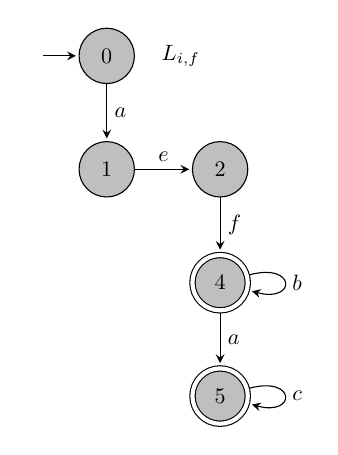
\begin{tikzpicture}
[->,>=stealth, node distance=18mm, auto, initial text=, on grid, shorten >=1pt,
every state/.style={fill=lightgray},
every node/.style={scale=0.8},
accepting/.style={double distance=1.5pt, outer sep=0.75pt+\pgflinewidth}
]
	\node[state, initial]	(0) 					{$0$};
	\node[state]			(1) [below of = 0]		{$1$};
	\node[state]			(2) [right of = 1]		{$2$};
	\node[state, accepting]	(4) [below of = 2]		{$4$};
	\node[state, accepting]	(5) [below of = 4]		{$5$};
	\node[right of = 0] at (-.5,0) {$L_{i,f}$};
	
  	\path
  		(0) edge 				node {$a$} (1)
  		(1) edge 				node {$e$} (2)
  		(2) edge 				node {$f$} (4)
  		(4) edge [loop right]	node {$b$} (4)
  		(4) edge 				node {$a$} (5)
  		(5) edge [loop right]	node {$c$} (5);
\end{tikzpicture}
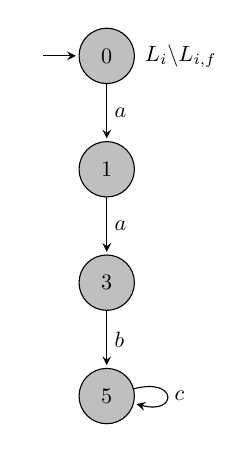
\begin{tikzpicture}
[->,>=stealth, node distance=18mm, auto, initial text=, on grid, shorten >=1pt,
every state/.style={fill=lightgray}, 
every node/.style={scale=0.8},
accepting/.style={double distance=1.5pt, outer sep=0.75pt+\pgflinewidth}
]
	\node[state, initial]	(0) 					{$0$};
	\node[state]			(1) [below of = 0]		{$1$};
% 	\node[state]			(2) [right of = 1]		{$2$};
	\node[state]			(3) [below of = 1]		{$3$};
% 	\node[state]			(4) [right of = 3]		{$4$};
	\node[state]			(5) [below of = 3]		{$5$};
	\node[right of = 0] at (-.5,0) {$L_i\backslash L_{i,f}$};
	
  	\path
  		(0) edge 				node {$a$} (1)
%   		(1) edge 				node {$e$} (2)
  		(1) edge 				node {$a$} (3)
%   		(3) edge 				node {$c$} (4)
  		(3) edge 				node {$b$} (5)
%   		(4) edge [loop right]	node {$b$} (4)
%   		(4) edge 				node {$a$} (5)
  		(5) edge [loop right]	node {$c$} (5);
\end{tikzpicture}
% \tikzset{align at top/.style={baseline=(current bounding box.north)}}
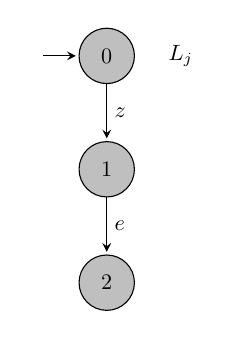
\begin{tikzpicture}
[->,>=stealth, node distance=18mm, auto, initial text=, on grid, shorten >=1pt,
every state/.style={fill=lightgray},
every node/.style={scale=0.8}, 
accepting/.style={double distance=1.5pt, outer sep=0.75pt+\pgflinewidth}
]
	\node[state, initial]	(0) 			{$0$};
	\node[state]			(1) [below of = 0]		{$1$};
	\node[state]			(2) [below of = 1]		{$2$};
	\node[right of = 0] at (-.5,0) {$L_j$};
	
  	\path
  		(0) edge 				node {$z$} (1)
  		(1) edge 				node {$e$} (2);
\end{tikzpicture}
% \caption{Automata representing faulty $L_{i,f}$ and
% non-faulty $L_i \backslash L_{i,f}$ languages of one module, and the language
% $L_j$ of a second module. Given $\Sigma_o = \{b, c, z\}$ the language $L_i
% \parallel L_j$ is not diagnosable.}
% \label{fig_changed_observation}
% \end{figure}
% 
% \begin{example} Consider one module the language $L_i$ as depicted in
% Figure \ref{fig_automaton_F-NF} and another module with a language $L_j$ as
% depicted in Figure \ref{fig_changed_observation}. At the last figure the
% only strings of $L_i$ which form indeterminate cycles are presented, assuming that 
% $\Sigma_o = \{b, c, z\}$. The language $L_i$ is not diagnosable since it has
% indeterminate cycle $\{bc^*\}$. If both $L_i$ and $L_j$ are composed
% (depicted in Figure \ref{fig_example_parallel}), then, as it
% stated in the Conjecture \ref{cnj_changed_observation}, all the string in
% $L_{i,f}$ change their observation.
% However, whenever the event $z$ is observed any string of $L_i\backslash
% L_{i,f}$ can be executed in the language $L_i \parallel L_j$.
% Thus, the composed system is not diagnosable either.
% \end{example}
% 
% The reason the observation changing does not affect diagnosability in the
% above example is that the non-faulty language $L_i\backslash L_{i,f}$ with its 
% strings which form indeterminate cycle are included in the inverse projection of
% $M(L_j)$, i.e.
% $
% L_i\backslash L_{i,f} \subseteq P_i^{-1}(M(L_j)).
% $
% Henceforth, we need to prohibit the execution of the observable event $z$
% in $L_j$ until some traces in $L_i$ are executed. The only way to do it is to
% make all the prefixes of the language $L'_j$ (defined in Conjecture
% \ref{cnj_changed_observation}) having common events, as it is shown in the
% following example.
% 
% \begin{figure}[t]
% \centering
% 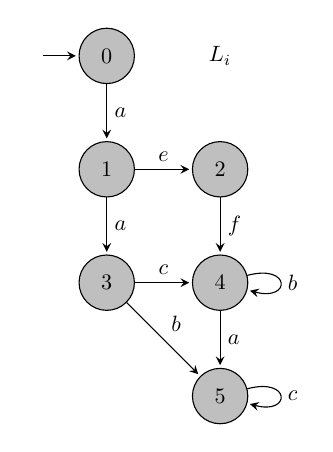
\begin{tikzpicture} 
[->,>=stealth, node distance=18mm, auto, initial text=, on grid,
shorten >=1pt, every state/.style={fill=lightgray}, 
every node/.style={scale=0.8}, 
accepting/.style={double distance=1.5pt, outer sep=0.75pt+\pgflinewidth}] 
	\node[state, initial]	(0) 					{$0$};
	\node[state]			(1) [below of = 0]		{$1$};
	\node[state]			(2) [right of = 1]		{$2$};
	\node[state]			(3) [below of = 1]		{$3$};
	\node[state]			(4) [right of = 3]		{$4$};
	\node[state]			(5) [below of = 4]		{$5$};
	\node[right of = 0] at (0,0) {$L_i$};
		
  	\path
  		(0) edge 				node {$a$} (1)
  		(1) edge 				node {$e$} (2)
  		(1) edge 				node {$a$} (3)
  		(2) edge 				node {$f$} (4)
  		(3) edge 				node {$c$} (4)
  		(3) edge 				node {$b$} (5)
  		(4) edge [loop right]	node {$b$} (4)
  		(4) edge 				node {$a$} (5)
  		(5) edge [loop right]	node {$c$} (5);
\end{tikzpicture}
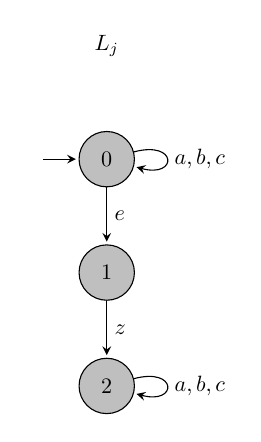
\begin{tikzpicture}
[->,>=stealth, node distance=18mm, auto, initial text=, on grid, shorten >=1pt,
every state/.style={fill=lightgray},
every node/.style={scale=0.8}, 
accepting/.style={double distance=1.5pt, outer sep=0.75pt+\pgflinewidth}
]
	\node[state, initial]	(0) 					{$0$};
	\node[state]			(1) [below of = 0]		{$1$};
	\node[state]			(2) [below of = 1]		{$2$};
	\node[above of = 0] at (0,0) {$L_j$};
	
  	\path
  		(0) edge [loop right]	node {$a, b, c$} (0)
  		(0) edge 				node {$e$} (1)
  		(1) edge 				node {$z$} (2)
  		(2) edge [loop right]	node {$a, b, c$} (2);
\end{tikzpicture}
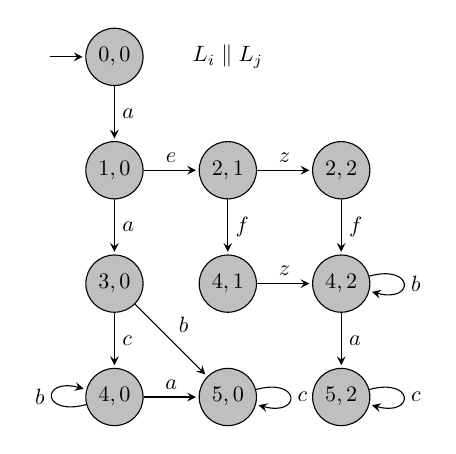
\begin{tikzpicture}
[->,>=stealth, node distance=18mm, auto, initial text=, on grid, shorten >=1pt,
every state/.style={fill=lightgray},
every node/.style={scale=0.8}, 
accepting/.style={double distance=1.5pt, outer sep=0.75pt+\pgflinewidth}
]
	\node[state, initial]	(00) 					{$0,0$};
	\node[state]			(10) [below of = 00]	{$1,0$};
	\node[state]			(21) [right of = 10]	{$2,1$};
	\node[state]			(22) [right of = 21]	{$2,2$};
	\node[state]			(41) [below of = 21]	{$4,1$};
	\node[state]			(42) [right of = 41]	{$4,2$};
	\node[state]			(52) [below of = 42]	{$5,2$};
	\node[state]			(30) [below of = 10]	{$3,0$};
	\node[state]			(40) [below of = 30]	{$4,0$};
	\node[state]			(50) [below of = 41]	{$5,0$};
 	\node[right of = 00] at (0,0) {$L_i \parallel L_j$};
	
   	\path
   		(00) edge 				node {$a$} (10)
   		(10) edge 				node {$e$} (21)
   		(10) edge 				node {$a$} (30)
   		(30) edge 				node {$c$} (40)
   		(30) edge 				node {$b$} (50)
   		(40) edge 				node {$a$} (50)
   		(21) edge 				node {$z$} (22)
   		(21) edge 				node {$f$} (41)
   		(22) edge 				node {$f$} (42)
   		(41) edge 				node {$z$} (42)
   		(50) edge [loop right]	node {$c$} (50)
   		(40) edge [loop left]	node {$b$} (40)
   		(42) edge [loop right]	node {$b$} (42)
   		(42) edge 				node {$a$} (52)
   		(52) edge [loop right]	node {$c$} (52);
\end{tikzpicture}
% \caption{Automata representing the language $L_i$ and the language $L_j$ which
% makes the language $L_i \parallel L_j$ diagnosable, given 
% $\Sigma_o = \{b, c, z\}$}
% \label{fig_changed_observation2}
% \end{figure}
% 
% \begin{example} In the Figure \ref{fig_changed_observation2} the language $L_i$
% has indistinguishable strings which form indeterminate cycle. The language
% $L_j$ satisfies the condition of the Conjecture \ref{cnj_changed_observation}
% since all the continuation of strings starting from the state $2$ have the
% observable event $z$ in the prefixes. Moreover, event $z$ does not occur until 
% event $e$ is executed. It can be checked, that the parallel composition of the
% languages $L_i$ and $L_j$ breaks indeterminate cycle, and the resulting
% language is diagnosable.
% 
% Note: The non-blocking assumption is violated in this particular example (for
% instance, 
% $\{a^*\} \in L_j$ but $\{a^*\} \not \in P^{-1}_j(L_i \parallel L_j)$).
% \end{example}
% 
% More formally, we require a set of strings 
% $\{\Sigma_j \sigma't\sigma''\} \subseteq L_j \mid \sigma', 
% \sigma'' \in \Sigma_i \cap \Sigma_j$ be observable: $M(t) \neq \emptyset$
% (this projection is equal to one define in \ref{cnj_changed_observation}),
% and all the common events be either in faulty or non-faulty sub-language of
% $L_i$, i.e 
% $$
% 	P_{i,j}^{-1}(L_j) \cap L_{i,f} = L_{i,f} \textrm{ or } 
% 	P_{i,j}^{-1}(L_j) \cap L_i\backslash \overline{L_{i,f}} 
% 	= L_i\backslash \overline{L_{i,f}}.
% $$
% The above condition is sufficient to make the system diagnosable. In other cases
% the compositional process is required.
% 
% In order to check the above requirements a verification procedure might be as
% follows (note, the complexity is linear):
% \begin{enumerate}
%   \item Mark the language $L_{i,f}$ by the automaton depicted in Figure
%   \ref{fig_marking_two_common}, left;
%   \item Mark the language $L_i\backslash \overline{L_{i,f}}$ the same way;
%   \item Check if only one marked language is not empty, and all strings of that
%   language reach the marked states. Continue if it is true, otherwise stop the
%   procedure;
%   \item Mark the language $L_j$ by the automaton depicted in Figure
%   \ref{fig_marking_two_common}, right;
%   \item If the marked language is not empty then declare the system is
%   diagnosable, otherwise declare the system is not diagnosable.
% \end{enumerate}
% 
% \begin{figure}[t]
% \centering
% \begin{tikzpicture}
% [->,>=stealth, node distance=18mm, auto, initial text=, on grid, shorten >=1pt,
% every state/.style={fill=lightgray},
% every node/.style={scale=0.8}, 
% accepting/.style={double distance=1.5pt, outer sep=0.75pt+\pgflinewidth}
% ]
% 	\node[state, initial]	(0) 				{$0$};
% 	\node[state]			(1) [below of = 0]	{$1$};
% 	\node[state, accepting]	(2) [below of = 1]	{$2$};
% 	\node[left of = 0] at (0,0) {$$};
% 
%   	\path
%   		(0) edge [loop right]
%   			node {$\Sigma_i \backslash (\Sigma_i \cap \Sigma_j)$} (0) 
%   		(0) edge
%   			node {$\Sigma_i \cap \Sigma_j$} (1) 
%   		(1) edge [loop right]
%   			node {$\Sigma_i \backslash (\Sigma_i \cap \Sigma_j)$} (1) 
%   		(1) edge
%   			node {$\Sigma_i \cap \Sigma_j$} (2) 
%   		(2) edge [loop right]
%   			node {$\Sigma_i $} (2); 
% \end{tikzpicture}
% \begin{tikzpicture}
% [->,>=stealth, node distance=18mm, auto, initial text=, on grid, shorten >=1pt,
% every state/.style={fill=lightgray},
% every node/.style={scale=0.8}, 
% accepting/.style={double distance=1.5pt, outer sep=0.75pt+\pgflinewidth}
% ]
% 	\node[state, initial]	(0) 				{$0$};
% 	\node[state]			(1) [below of = 0]	{$1$};
% 	\node[state]			(2) [below of = 1]	{$2$};
% 	\node[state, accepting]	(3) [below of = 2]	{$3$};
% 	\node[left of = 0] at (0,0) {$$};
% 
%   	\path
%   		(0) edge [loop right]
%   			node {$\Sigma_j \backslash (\Sigma_i \cap \Sigma_j)$} (0) 
%   		(0) edge
%   			node {$\Sigma_i \cap \Sigma_j$} (1) 
%   		(1) edge [loop right]
%   			node {$\Sigma_j \backslash (\Sigma_o \backslash (\Sigma_i \cap	\Sigma_j))$} (1) 
%   		(1) edge
%   			node {$\Sigma_o \backslash (\Sigma_i \cap	\Sigma_j)$} (2) 
%   		(2) edge [loop right]
%   			node {$\Sigma_j \backslash (\Sigma_i \cap \Sigma_j)$} (2) 
%   		(2) edge
%   			node {$\Sigma_j \cap \Sigma_j$} (3) 
%   		(3) edge [loop right]
%   			node {$\Sigma_j $} (3); 
% \end{tikzpicture}
% \caption{Automata for marking the languages $L_i$ and $L_j$}
% \label{fig_marking_two_common}
% \end{figure}
% 
% We proceed by establishing a necessary condition for diagnosability by an
% adjacent module. The non-blocking assumption is relaxed in the following.
% Firstly we define a \emph{potentially non-blocking} string for the language of
% an adjacent module:
% 
% \begin{definition} A string $s \in L_j$ is potentially non-blocking with respect
% to any string from $L_i$ if there is no a string with more then two common events
% in it, and the common event is in the strongly connected component, i.e:
% $$
% \begin{array}{l}
% 	(\forall \sigma, \sigma' \in \Sigma_i \cap \Sigma_j \mid \sigma \neq
% 	\sigma') 
% 	[\not \exists ~\Sigma_j \sigma \Sigma_j \sigma' \in \overline{s}]
% 	\textrm{ and} \\
% 	(\forall ~\Sigma_j \sigma \in \overline{s}) 
% 	[\exists \Sigma_j \sigma t \in \overline{s} \mid \Sigma_j \sigma \in \overline{t}]
% 	
% \end{array}
% $$
% \end{definition}
% Consequently, a \emph{potentially blocking} string is a string which has more
% then one common events in it, or the common event is not in a strongly connected
% component. It worth noting that this definition has no assumptions about the
% strings of the language $L_i$. However, there are conditions of non-blocking
% when the structure of both languages is known. For instance, the case when 
% languages have strings with one common event and this event is in a strongly
% connected component or not, equally for both languages. These cases reflected in
% the two conjectures below (skip them to proceed to a more general condition).
% 
% \begin{conjecture}[SCC with one common event] If an adjacent module has a
% common event only in its strongly connected component (SCC), and that event is
% common only to events in the indeterminate cycle (which is a SCC as well), then
% the composition does not change the diagnosability property.
% \end{conjecture} 
% 
% The proof of the above conjecture seems trivial, since any prefix of the
% adjacent module's SCC before the common event forms an interleaving with the
% language of non-diagnosable module. And the SCC itself is projected to the only
% state with respect to the common event, no matter how many observable
% events the SCC has.
% 
% \begin{conjecture}[SCC with many common events] If an adjacent module has 
% common events only in its strongly connected component (SCC), and those events
% are common only to events in the indeterminate cycle (which is a SCC as well),
% then the composition does not change the diagnosability property.
% \end{conjecture}
% 
% In the above conjecture if the both SCC have the same projection with respect to
% the common events then the indeterminate cycle is not changing. Otherwise it
% might be or not changed due to blocking. Nevertheless, the observable
% projection of the adjacent SCC changes an observable projection of
% the indeterminate cycle equally for both faulty and non-faulty strings.
% 
% A weakest, most general condition for changing diagnosability by an
% adjacent module is the next:
% 
% \begin{conjecture}[Necessary condition for changing diagnosability] Given two
% languages $L_i$ and $L_j$, and the a faulty behaviour is defined only for $L_i$.
% Diagnosability property of $L_i$ can be changed by the parallel composition $L_i
% \parallel L_j$ only if the language $L_j$ has a potentially blocking string with
% respect to another language.
% % \begin{equation}
% % L_{j,s}^{>1} \neq \emptyset
% % \end{equation}
% \end{conjecture}
% In the above, $L_{j,s}^{>1} \neq \emptyset \Rightarrow L_{i,s}^{1} \neq \emptyset$ 


% $$
% \begin{array}{l}
% 	P_{i,j}^{-1}(L_{i,f}) \cap P_{i,j}^{-1}(L_i \backslash L_{i,f})
% \end{array}
% $$



% From the above we can see that the assumption of Contant that the common events
% are observable, actually does not affect the observability property.

%%%%%%%%%%%%%%%%%%%%%%%%%%%%%%%%%%%%%%%%%%%%%%%%%%%%%%%%%%%%%%%%%%%%%%%%%%%%%%%
% \section{todo:}
% \begin{enumerate}
%   \item Who defines the models of the components? 
%   \item What exactly makes modular diagnoses different from each other?
%   \item Check for approaches where the number of diagnosers varies.
% \end{enumerate}
% \begin{figure}[ht]
% \centering
% 	\includegraphics[height=95mm]{parallel.jpg}
% 	\caption{The result of the parallel composition of the languages depicted in
% 	Figure \ref{fig_changed_observation} (Looks ugly? Thanks DESUMA)}
% 	\label{fig_example_parallel}
% \end{figure}



% \newpage
% \section{Excluded from the paper but might be useful}
% \begin{figure}[ht]
% \centering
% 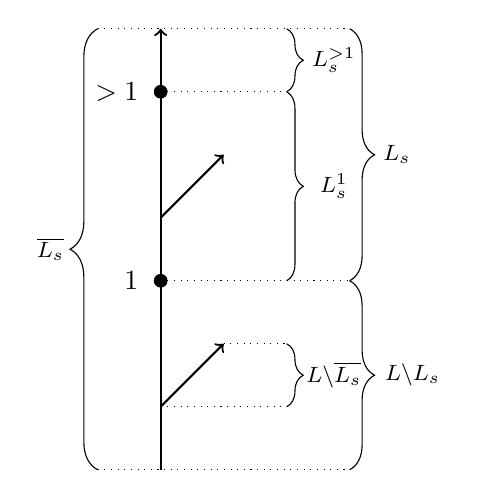
\begin{tikzpicture}[scale=.8]
\draw [thick] [->](2,1)--(2,8);
\draw [thick] [->](2,2)--(3,3);
\draw [thick] [->](2,5)--(3,6);
% Events
\draw [fill] (2,4) circle [radius=0.1];
\node [left] at (1.8,4) {$1$};
\draw [fill] (2,7) circle [radius=0.1];
\node [left] at (1.8,7) {$>1$};
% Braces
\draw [decorate,decoration={brace,amplitude=10pt}]
 	(1,1)--(1,8) node [midway,xshift=-0.6cm] {\footnotesize $\overline{L_s}$};
\draw [decorate,decoration={brace,amplitude=6pt}]
 	(4,8)--(4,7) node [midway,xshift=0.6cm] {\footnotesize $L^{>1}_s$};
\draw [decorate,decoration={brace,amplitude=6pt}]
 	(4,7)--(4,4) node [midway,xshift=0.6cm] {\footnotesize $L^{1}_s$};
\draw [decorate,decoration={brace,amplitude=9pt}]
 	(5,8)--(5,4) node [midway,xshift=0.6cm] {\footnotesize $L_s$};
\draw [decorate,decoration={brace,amplitude=6pt}]
 	(4,3)--(4,2) node [midway,xshift=0.6cm] {\footnotesize $L \backslash
 	\overline{L_s}$};
\draw [decorate,decoration={brace,amplitude=9pt}]
 	(5,4)--(5,1) node [midway,xshift=0.8cm] {\footnotesize $L \backslash L_s$};
%Dashed lines
\draw [dotted] (1,8)--(5,8);
\draw [dotted] (2,7)--(4,7);
\draw [dotted] (2,4)--(5,4);
\draw [dotted] (3,3)--(4,3);
\draw [dotted] (2,2)--(4,2);
\draw [dotted] (1,1)--(5,1);
\end{tikzpicture}
% \caption{Structural schema of the definition of the synchronized language
% $L_s$ over a language $L$}
% \label{fig_partitioning_synch}
% \end{figure}
% 
% For the sake of clarity we introduce a structural schema of the
% synchronized language defined by \ref{eq_synchronized_language} in Section
% \ref{sec:definitions}. It is depicted in Figure \ref{fig_partitioning_synch}.
% (In the figure the language $L_s$ is equal to $L'$ in \ref{sec:definitions}).

\end{document}
